%-*-    coding: UTF-8   -*-
\documentclass[UTF-8]{ctexart}

\usepackage{graphicx}
\usepackage{subfigure}
\usepackage{amsmath}
\usepackage{geometry}%页面设置
\usepackage{tabularx}%表格扩展
\usepackage{color}
\usepackage{xcolor}
\usepackage{hyperref}
\usepackage{ulem}
\usepackage{multirow}%表格合并
\usepackage{amsmath}%数学公式
\usepackage{longtable}%表格跨页
%\usepackage[cache=false]{minted}%代码高亮
\usepackage{fontspec,xunicode,xltxtra}
\usepackage{fontspec}%字体设置
\usepackage{authblk}%作者设置
\usepackage{booktabs}
\usepackage{cite}%文献引用
\usepackage{float}
%\usepackage{figure}
%取消链接的红框
\hypersetup{
	colorlinks=true,
	linkcolor=black,
	citecolor=gray
}

%A4纸大小,版心居中,长宽占页面的0.8
\geometry{a4paper,centering,scale=0.8}
%改变图表标题格式,此处使用悬挂对齐方式(编号向左突出),小字号,标题使用斜体
\usepackage[format=hang,font=small,textfont=it]{caption}
%增加目录项目,tocbibind宏包会自动加入目录项本身、参考文献、索引等项目。[nottoc]取消了对自身的显示
\usepackage[nottoc]{tocbibind}

%定义代码高亮,方便下面编写
\definecolor{bg}{rgb}{0.95,0.95,0.95}
%\newcommand{\cpp}[1]{\inputminted[bgcolor=bg,breaklines,breakanywhere=true]{c++}{#1}}


%字体声明,等宽字体采用 Consolas ()Ubuntu Mono)
\setmonofont{Consolas}

%title 信息
\title{不围棋报告}
\author{2000012983 宋聿辰}
\date{\today}
\affil{北京大学信息科学技术学院}

\begin{document}
	\maketitle%输出题目
	\begin{abstract}
	\end{abstract}
	\newpage
	\tableofcontents%输出目录
	\newpage%换页
	\section{不围棋介绍}
		与围棋相反,不围棋的胜利目标是想方设法不要让自己提走对方的棋子,而要尽可能的让自己的棋子被对方提走。与一个棋子直线相邻的空点称为“气”,相邻同色棋子的“气”一并计算。当一个棋子没有“气”的时候它就要被提走。
		\begin{figure}[H]
			\centering
			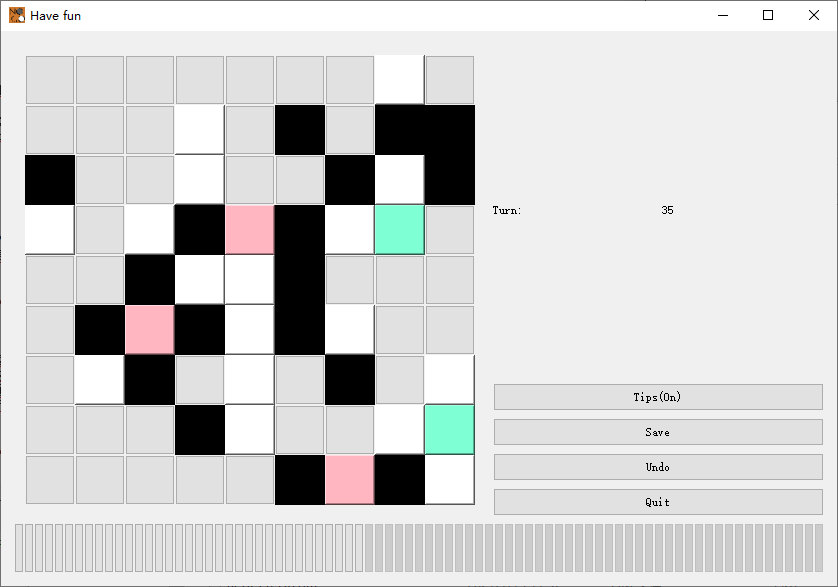
\includegraphics[width=15cm]{./file/main.png}
			\caption{不围棋}
		\end{figure}
	\section{AI算法}
		共设计了三个不同梯度的 AI 算法:随机算法,贪心算法,蒙特卡洛搜索树算法(MCTS)。
		\subsection{随机算法}
		排除所有不能下的位置,把剩下的所有能下的位置挑选出来,随机地选择一个。
		为了保证随机性,使用 Mersenne Twister 算法生成随机数。这种算法随机性很好,且在计算机上比较容易实现,产生随机数地速度较快,周期长。
		\begin{figure}[H]
			\centering
			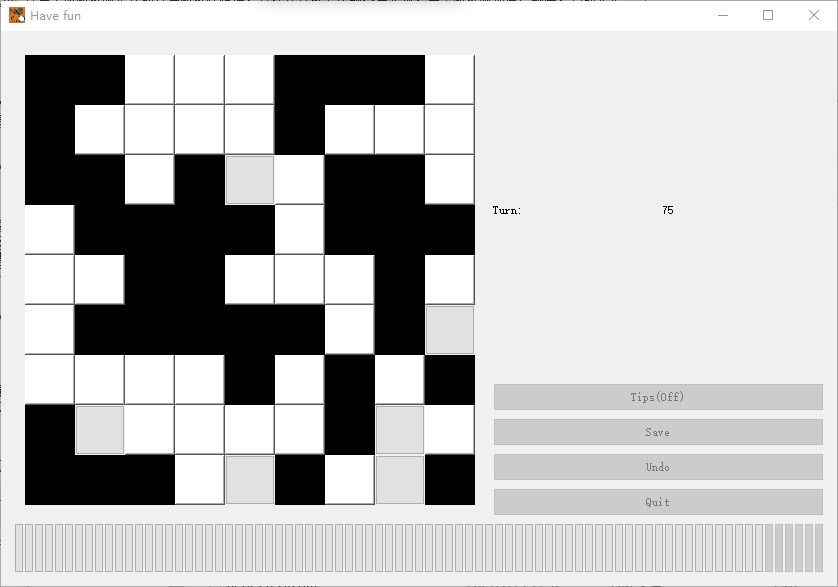
\includegraphics[width=13cm]{./file/random.png}
			\caption{随机算法}
		\end{figure}
		\subsection{贪心算法}
			考虑人类玩家的一般策略,即做“眼”,故对棋盘上可能形成“眼"的位置设置更高的权重,使用累加的方法,按照权重进行随机选择。从表现来看,贪心算法倾向于在棋盘上下出网格,以最大化眼的数量。
			\begin{figure}[H]
				\centering
				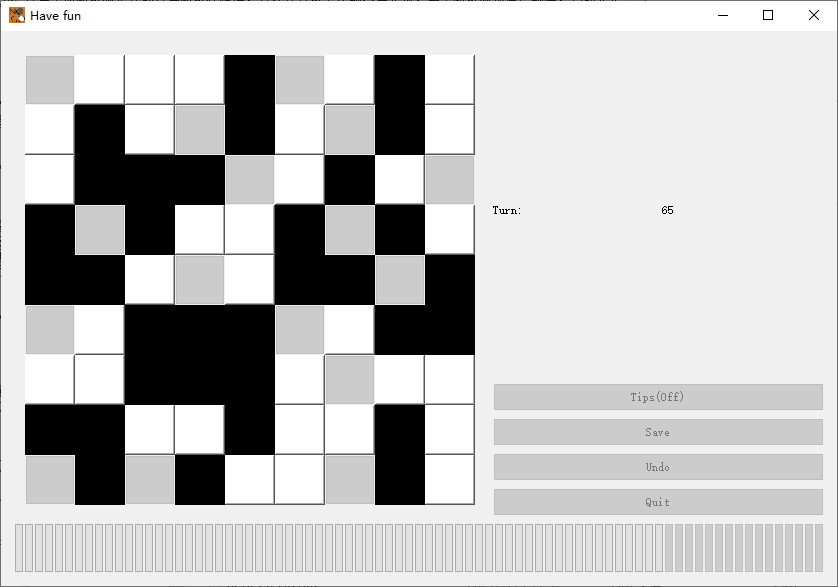
\includegraphics[width=13cm]{./file/greedy.png}
				\caption{贪心算法}
			\end{figure}
		\subsection{MCTS}
			蒙特卡洛搜索树算法是对传统的搜索算法的优化,它平衡了传统搜索中广度和深度的权衡,使在不能搜索整个搜索树的时候,采用一定的策略,搜索一定数量的部分节点,从概率的角度作出决策。
			具体来说,该算法采用上限置信区间算法(UCT)来决定在树上每一步的走法,如果走到了一个空节点即该棋盘走法尚未探索过,则开始随机走子直到得到一个终局局面,然后回溯更新所有的祖先信息。重复该过程若干次后,选择最优的节点作为该局的落子。
			\begin{figure}[H]
				\centering
				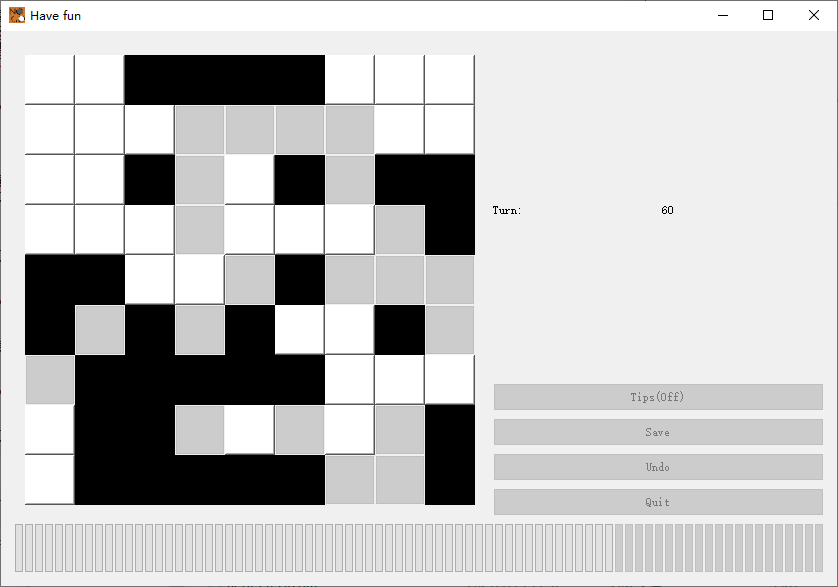
\includegraphics[width=13cm]{./file/mcts.png}
				\caption{MCTS 算法}
			\end{figure}
	\section{具体实现}
		\subsection{核心功能}
			棋盘上,落子和终局的判定采用并查集来实现。具体来说,对于每一个并查集的根维护它所在的连通块的“气”。当放置一个新的棋子时,更新相邻连通块的“气”的信息,终局判定也是一样。
			鉴于在游戏功能中有撤回功能且 AI 算法中涉及到回溯,这里的并查集采用可持久化的方式进行维护,单次操作的复杂度为 $O(n\log n)$。
		\subsection{界面布局}
			采用 Qt 进行界面设计和布局。
			主窗口是开始新棋局、加载存档和切换语言的入口。
			\begin{figure}[H]
				\centering
				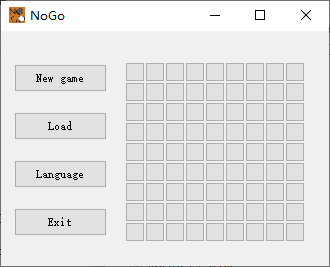
\includegraphics[width=7cm]{./file/mainw.png}
				\caption{主窗口}
			\end{figure}
			主棋盘界面负责实现棋局对局的所有主要功能。
			\begin{figure}[H]
				\centering
				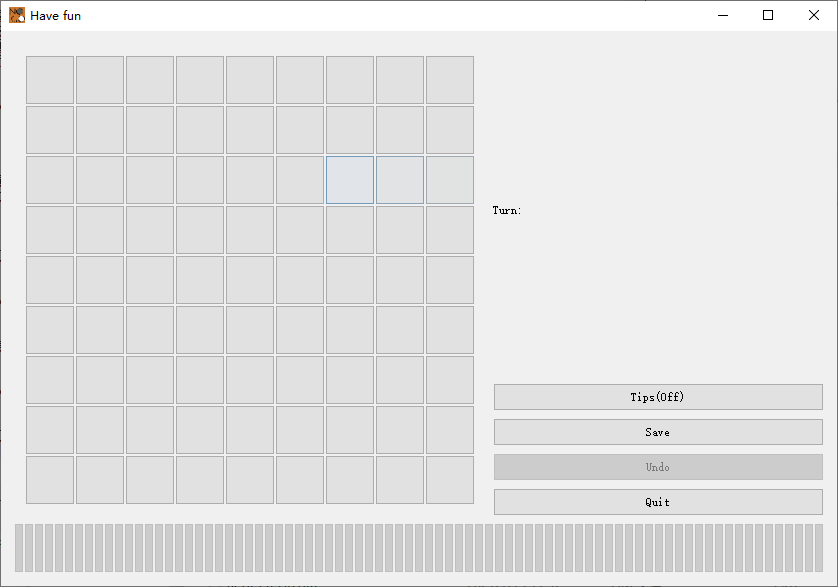
\includegraphics[width=13cm]{./file/playw.png}
				\caption{主棋盘界面}
			\end{figure}
			另外还有两个小的消息框负责语言切换和对弈双方的设定。
			\begin{figure}[H]
				\centering
				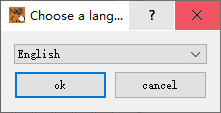
\includegraphics[width=7cm]{./file/language.png}
				\caption{语言切换}
			\end{figure}
			\begin{figure}[H]
				\centering
				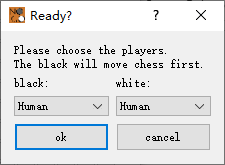
\includegraphics[width=7cm]{./file/player.png}
				\caption{对弈双方设定}
			\end{figure}
		\subsection{特性功能}
			\subsubsection{历史回放}
				支持在对弈的任意时刻查看之前双方下过的棋子,点击在棋盘下方的进度条可以临时地回溯到之前某一时刻的棋盘情况。
			\subsubsection{落子提示}
				在棋盘的右边有落子提示开关,默认是关闭的。开关打开后,会在棋盘中用两种颜色进行提示,被红色标记的格子意为当前执子方不能落子的位置,被绿色标记的格子意为当前执子放能落子但对方不能落子的位置。这些提示可以更好地帮助对弈双方进行决策。
			\subsubsection{撤回}
				在除终局以外的任意时刻均可以进行撤回操作。当双方中有一方为电脑玩家时,同时撤回双方的各一步;当双方均为人类玩家时,撤回只撤回当前执子方的一步。
			\subsubsection{存档和读档}
				支持在除终局以外的任意时刻进行存档,在主界面读档以恢复棋盘。
			\subsubsection{国际化}
				支持简体中文和英文两种语言。
	%\bibliographystyle{plain}
	%\bibliography{reference}
\end{document}